\documentclass[a4paper,11pt,twoside,openright]{book}							% COMANDI INIZIALI
\usepackage[italian]{babel}								% sillabazione italiana
\usepackage[utf8]{inputenc}								% Per le lettere accentate IN UNIX E IN WINDOWS
\usepackage{ragged2e}					 				% giustifica
\usepackage{amsmath}									% Per allineare le equazioni
\usepackage{amssymb}									% Per le lettere dell'indicatrice (mathbb)

\usepackage{graphicx}
\usepackage{amsthm}
\usepackage{amssymb}
\usepackage{amsmath}
\usepackage{mathtools}
\usepackage{caption}
\usepackage{booktabs}
\usepackage{hyperref}
\usepackage{float}
\usepackage{subfigure}
\usepackage{multirow}						% Per le tabelle di gcv, multiple row
\usepackage{array}							% Per avere i separatori di colonna più spessi

\justifying 										% giustifica

\date{28 Luglio 2014}
\author{Gabriele Mazza}
\title{Simulazione Dominio a C}

\begin{document}

%Indice e numerazione
\pagenumbering{arabic}

\chapter{Simulazione del codice}

Prima di provare il modello sul dominio della provincia di Venezia sono state eseguite delle prove su un caso noto e più semplice. Si è scelto il dominio a forma di C e la corrispondente funzione spaziale $g$ descritti in CITAZIONE NECESSARIA e nel pacchetto R \textit{mgcv} (in figura \ref{fig:domC_fstest}), e si è introdotta una variazione temporale deformando con il coseno:
$$
f(\underline p, t)=g(\underline p)cos(t)
$$
Su questo semplice caso sono stati eseguiti i primi tentativi.


\section{Triangolazione e istanti temporali}
Non sono presenti in questo caso punti spaziali definiti dalla natura del problema (come possono essere i comuni per la provincia di Venezia), quindi è stato necessario ricavarli. Sono stati generati casualmente 150 punti all'interno del rettangolo $(-1,+3.5) \times (-1,+1)$, e di questi sono stati considerati validi solo quelli che ricadevano all'interno del dominio. Non è stata usata la descrizione della frontiera presente in \textit{mgcv}, ma una versione diversa che permette di avere punti anche nella parte rettilinea del bordo.
\begin{figure}[!t]
\centering
\subfigure[Funzione spaziale $g(\underline p)$]
   {
   \label{fig:domC_fstest}
	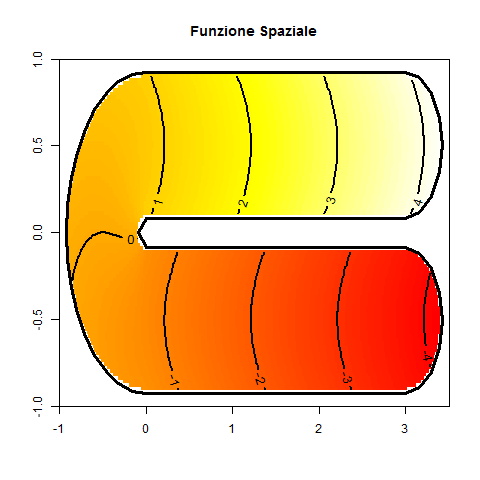
\includegraphics[width=0.46\textwidth]{Immagini/DomC_fstest.png}   
   }
\subfigure[Triangolazione]
   {
   \label{fig:domC_triang}
	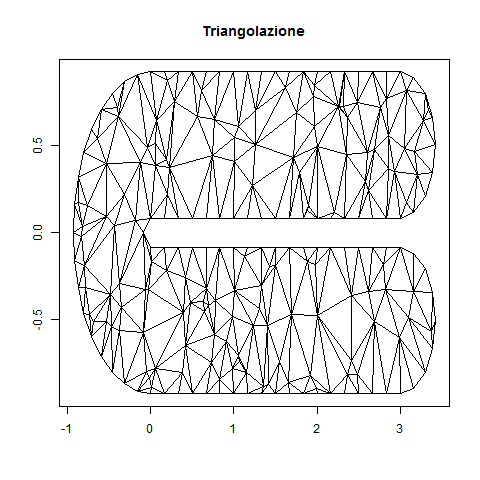
\includegraphics[width=0.46\textwidth]{Immagini/DomC_Triangolazione.png}
   }
\caption{Dominio a forma di C}
\label{fig:domC}
\end{figure}
In figura \ref{fig:domC_triang} è riportata la triangolazione ottenuta grazie al pacchetto R \textit{RTriangle}. In tutti gli esempi che seguiranno sarà considerata questa descrizione del dominio, che è formata da 241 punti (133 interni, 108 di frontiera) e 372 triangoli.

Come intervallo temporale di variazione dei dati è stato scelto $[0,2\pi]$, per sfruttare la periodicità del coseno. All'interno di questo intervallo sono stati ricavati 9 istanti temporali equidistanti tra di loro, quindi uno ogni $\frac{\pi}{4}$.

\section{Caso senza covariate}
Come primo passo è necessario scegliere i valori per $\lambda$ ottimizzando l'indice $\mathrm{GCV}(\underline \lambda)$ come riportato in RIMANDO NECESSARIO. In queste analisi $\lambda_S$ e $\lambda_T$ sono sempre espressi in potenze di 10. Dopo aver creato una griglia di valori in spazio e tempo, è stato ricercato il minimo sulla griglia. Il procedimento è stato eseguito più volte, rendendo la griglia sempre più fitta. In particolare, nel primo caso i valori sono distanziati di 1, poi (una volta che è possibile centrare gli intervalli in base al risultato precedente) di 0.25 e 0.125.

\begin{table}[htbp]
\renewcommand{\arraystretch}{1.3}
\setlength{\tabcolsep}{2mm}
\centering
	\begin{tabular}{!{\vrule width 1.2pt}c!{\vrule width 1.2pt}c!{\vrule width 1.2pt}}
	\noalign{\hrule height 1.2pt}
	Intervalli per $\lambda_S$ e $\lambda_T$& Miglior valore											\\
	\noalign{\hrule height 1.2pt}
	$\lambda_S \in \{-5,-4,\ldots,+1\}$ 	& \multirow{2}{*}{$\underline \lambda = (0,-3)$} 			\\
	\cline{1-1}
	$\lambda_T \in \{-5,-4,\ldots,+1\}$		& 															\\	
	\noalign{\hrule height 1.2pt}
	$\lambda_S \in \{-1,-0.75,\ldots,+1\}$ 	& \multirow{2}{*}{$\underline \lambda = (-0.5,-3.25)$} 		\\
	\cline{1-1}
	$\lambda_T \in \{-4,-3.75,\ldots,-2\}$	& 															\\	
	\noalign{\hrule height 1.2pt}
	$\lambda_S \in \{-1,-0.875,\ldots,+0\}$ 	& \multirow{2}{*}{$\underline \lambda = (-0.375, -3.25)$}	\\
	\cline{1-1}
	$\lambda_T \in \{-3.75,-3.625,\ldots,+2.75\}$		& 												\\	
	\noalign{\hrule height 1.2pt}
	\end{tabular}
\caption{Analisi di $\mathrm{GCV}(\underline \lambda)$}
\end{table}

L'analisi è stata eseguita con $\underline \lambda = (-0.375, -3.25)$. I dati sono stati generati aggiungendo al valore vero (facilmente ricavabile, potendo conoscere $g(\underline p)$) in ogni punto) un rumore generato da una normale di media nulla e deviazione standard $\sigma$ pari a 0.5.

\begin{figure}[t]
\centering
\subfigure[Funzione reale a $t=0$]
   {
	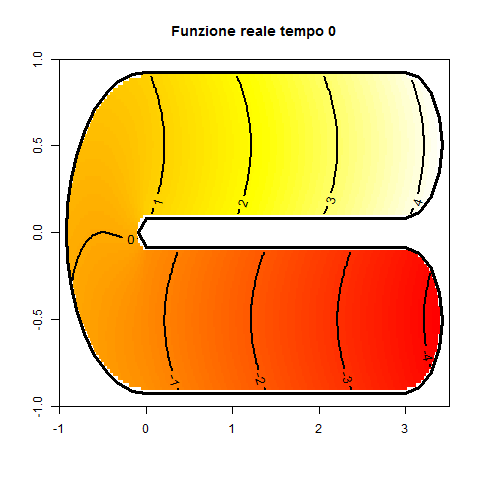
\includegraphics[width=0.46\textwidth]{Immagini/DomC_0reale.png}   
   }
\subfigure[Funzione stimata a $t=0$]
   {
	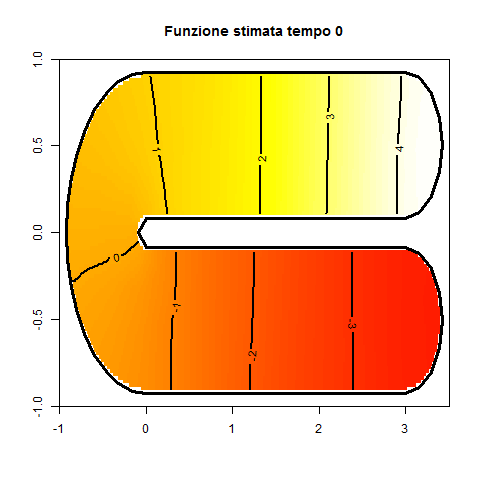
\includegraphics[width=0.46\textwidth]{Immagini/DomC_0stimata.png}
   }
\subfigure[Funzione reale a $t=\frac{\pi}{4}$]
   {
	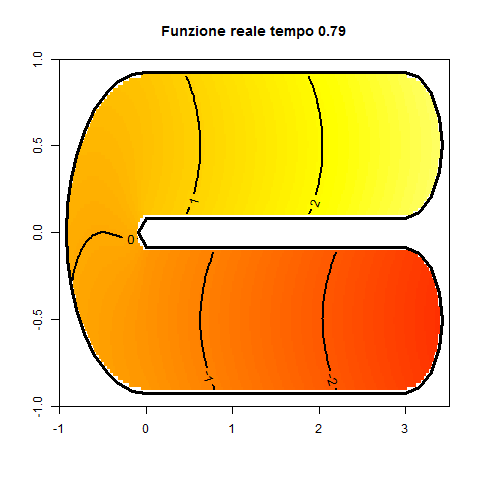
\includegraphics[width=0.46\textwidth]{Immagini/DomC_pi4reale.png}   
   }
\subfigure[Funzione stimata a $t=\frac{\pi}{4}$]
   {
	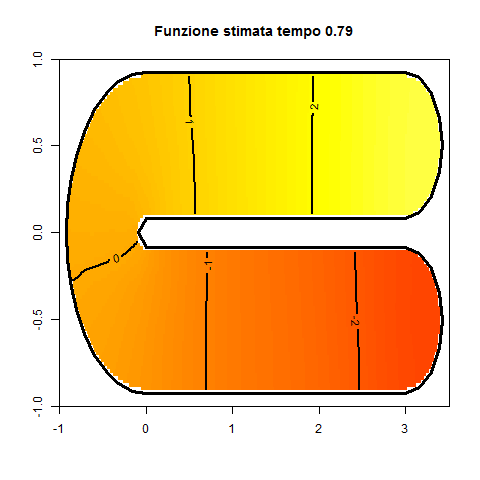
\includegraphics[width=0.46\textwidth]{Immagini/DomC_pi4stimata.png}
   }
\subfigure[Funzione reale a $t=\frac{\pi}{2}$]
   {
	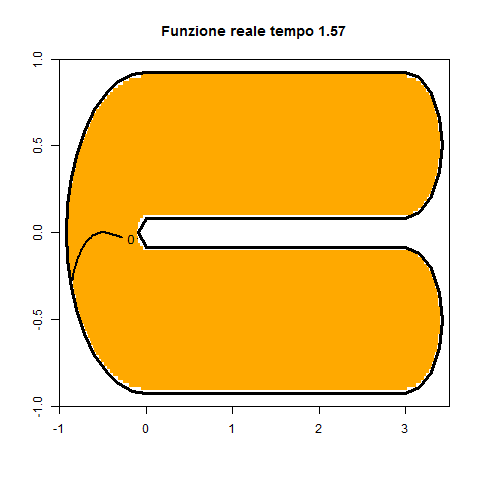
\includegraphics[width=0.46\textwidth]{Immagini/DomC_pi2reale.png}   
   }
\subfigure[Funzione stimata a $t=\frac{\pi}{2}$]
   {
	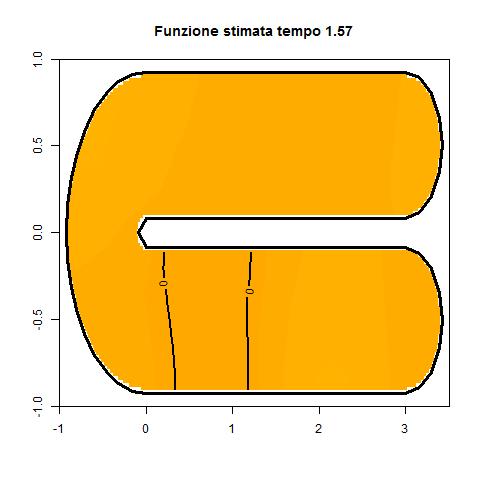
\includegraphics[width=0.46\textwidth]{Immagini/DomC_pi2stimata.png}
   }
\caption{Stime della funzione $f(\underline p,t)$ ad alcuni istanti di tempo}
\label{fig:DomC_ris}
\end{figure}

La stima della funzione si è rivelata molto buona. In figura \ref{fig:DomC_ris} si riportano i confronti tra funzione reale e stimata in alcuni istanti di tempo (la scala di colori è stata resa uniforme tra tutti i grafici). Si può notare come la funzione stimata sia effettivamente molto simile a quella reale. 

\begin{figure}[t]
\centering
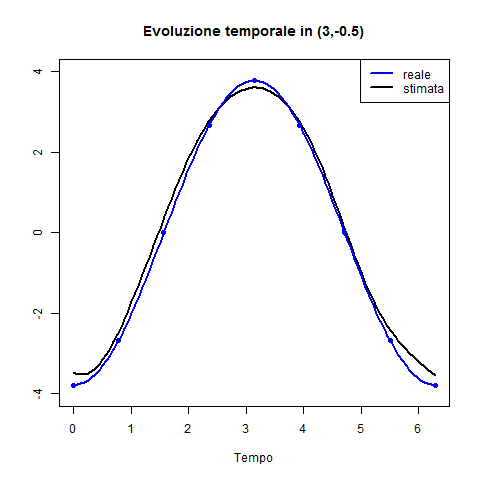
\includegraphics[width=0.46\textwidth]{Immagini/DomC_tfissato.png}   
\label{fig:DomC_ris2}
\end{figure}



\end{document}